\section{Results Inspection \& Analysis}
\label{sec:eval_inspect}

As described before, there are several levels of detail in which sub-results can be inspected.\\

The uppermost is the 'Requirements$\rightarrow$Overview', giving the sector sums for all requirements. \\

The next level of detail are the sector sum details, located in 'Sectors$\rightarrow$Sector Layer Name$\rightarrow$Requirement Group Name$\rightarrow$Requirement Name'. \\

The lowest level are the per-target details, located in 'Targets$\rightarrow$UTN' and the respective per-target results located in 'Targets$\rightarrow$UTN$\rightarrow$Sector Layer Name$\rightarrow$Requirement Group Name$\rightarrow$Requirement Name'. \\

By default, when single-clicking a row in a table the respective results are shown in the existing Views. When double-clicking, a step into the next level of detail is performed (if available). \\

Navigation can be made more efficient by returning to the last sub-result by using the 'Back' button on the top-left. \\

Different requirement results may use different views to display additional result details for deeper inspection:

\begin{itemize}  
\item Geographic View
\begin{itemize}  
\item Overview grid: 2D grid showing all grid cells with at least 1 issue as red, green otherwise
\item Per-target issue display: Mark test target reports with issues with red border, green otherwise
\end{itemize}
\item Histogram Views
\begin{itemize}  
\item Show counts of \#OK and \#NotOK, or numerical distribution of e.g. calculated error/offset
\end{itemize}
\end{itemize}
\ \\

\subsection{Results Overview}
\begin{figure}[H]
  \hspace*{-2cm}
    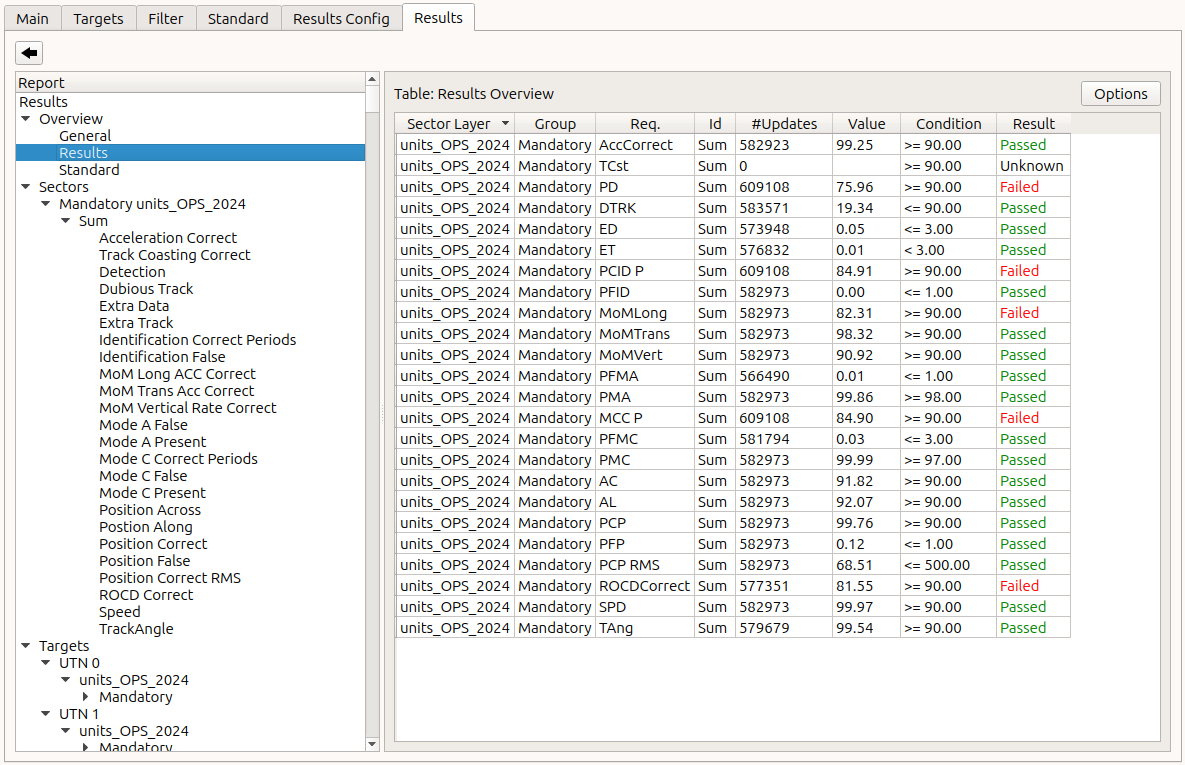
\includegraphics[width=18cm,frame]{figures/eval_results_overview.png}
  \caption{Evaluation results: Overview}
\end{figure}

Please note that the results are given as example only and are no indication of performance for any system currently in operation. \\

When single-clicking a row, the respective sector requirement results are shown in the existing Views.

\begin{figure}[H]
  \hspace*{-2.5cm}
    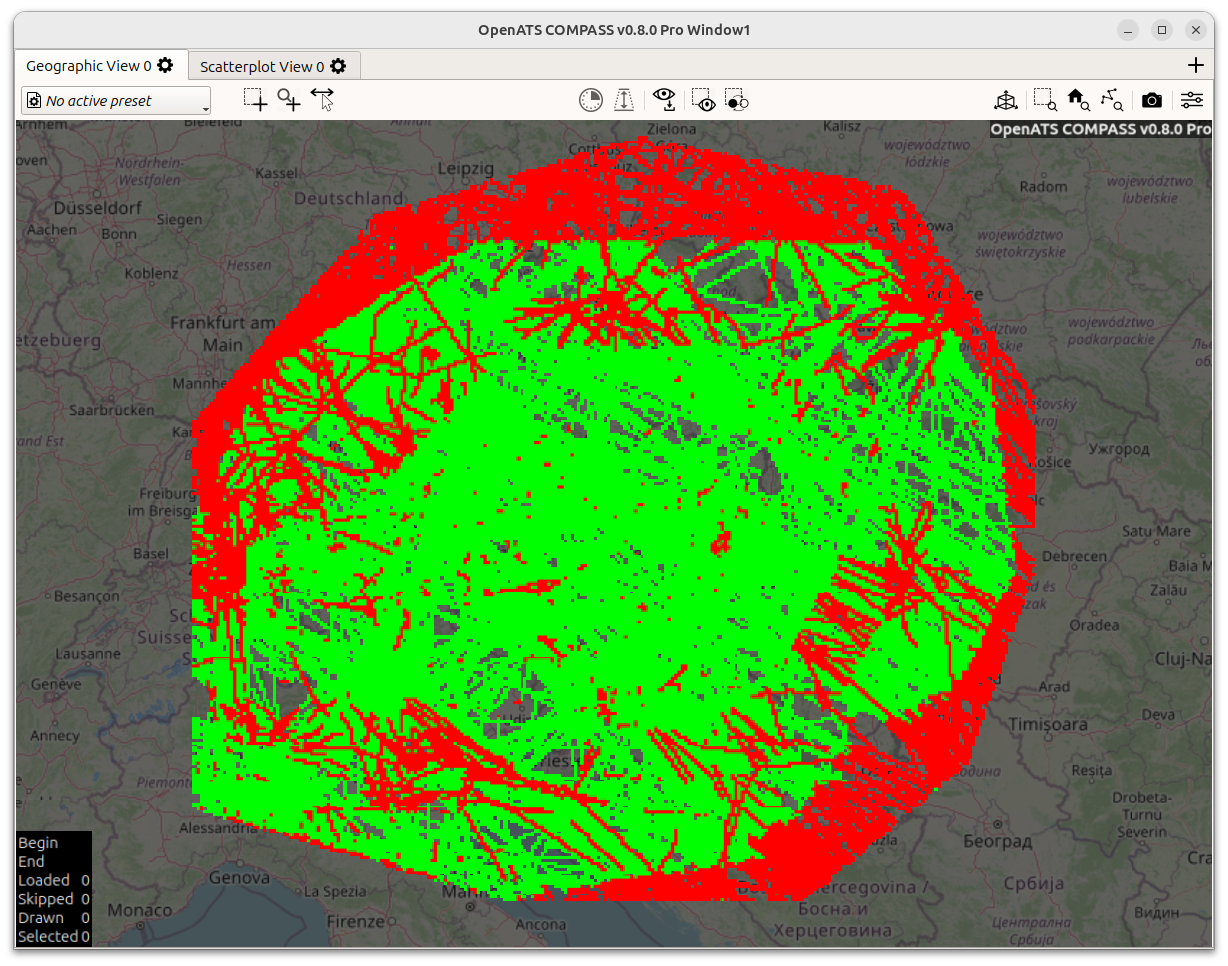
\includegraphics[width=19cm]{figures/geo_eval_detection.png}
  \caption{Evaluation Results: Detection in Geographic View}
\end{figure}

\begin{figure}[H]
  \hspace*{-2.5cm}
    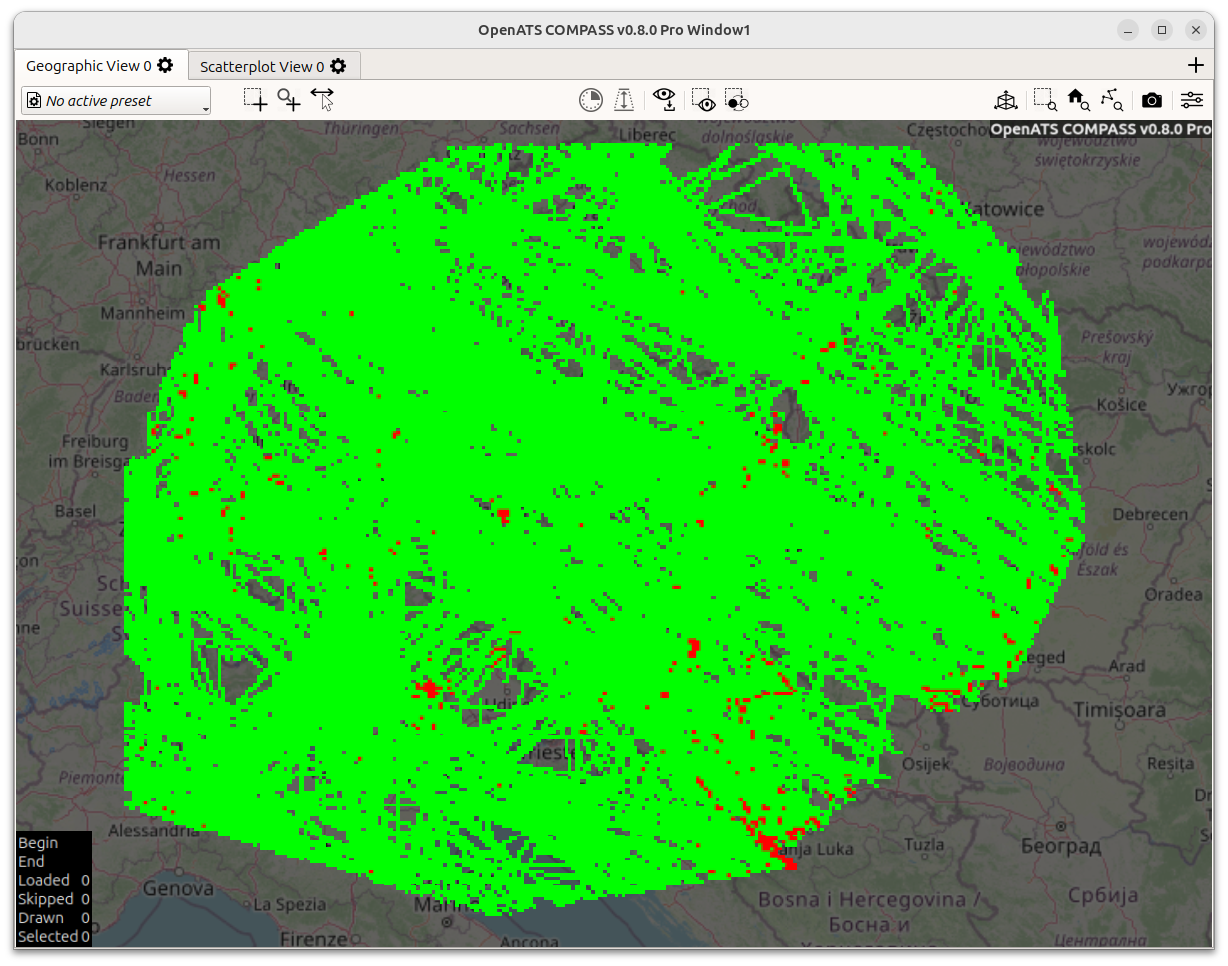
\includegraphics[width=19cm]{figures/geo_eval_pos_correct.png}
  \caption{Evaluation Results: Position Correct in Geographic View}
\end{figure}

\begin{figure}[H]
  \hspace*{-2.5cm}
    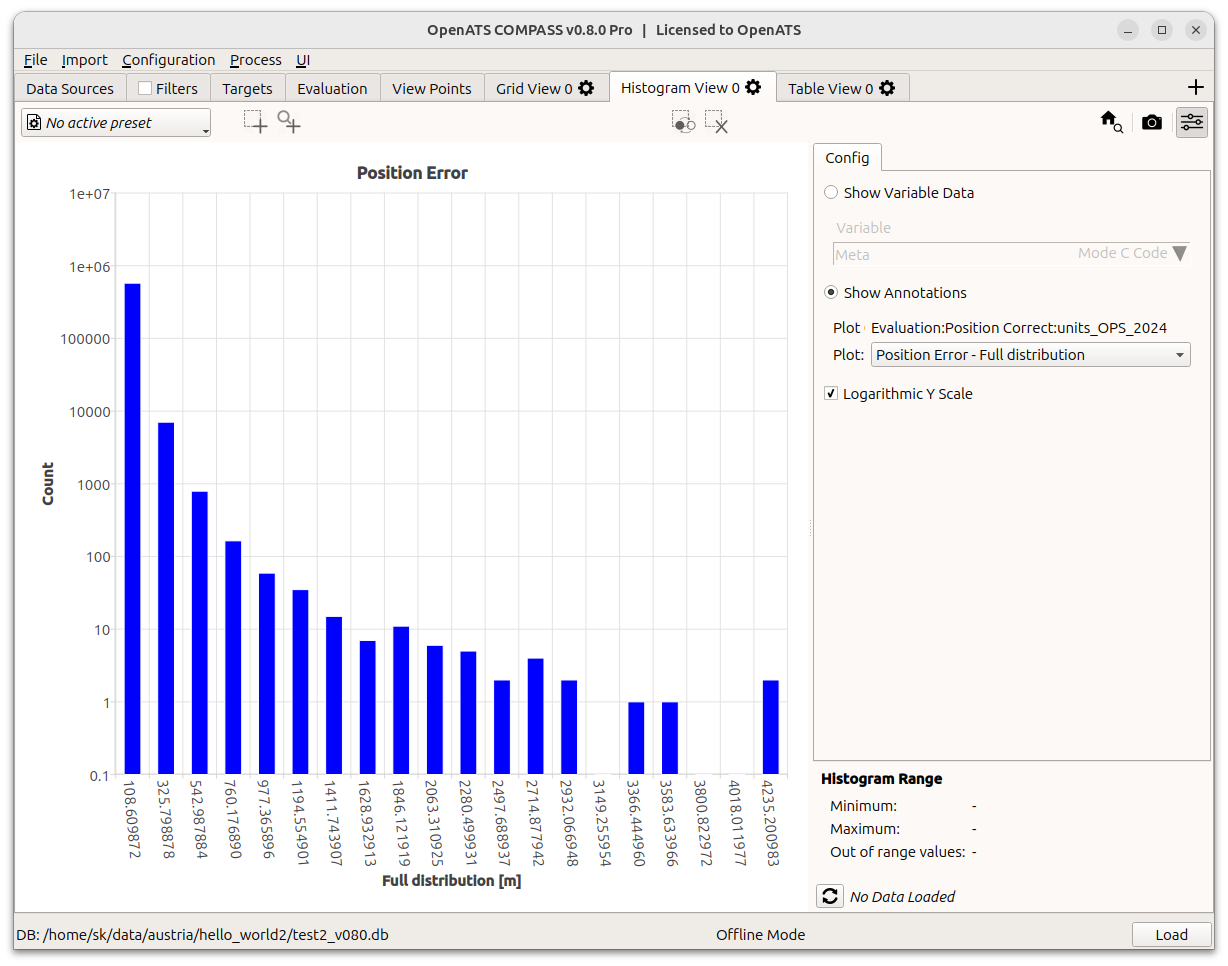
\includegraphics[width=19cm]{figures/histogram_eval_pos_correct.png}
  \caption{Evaluation Results: Position Correct in Histogram View}
\end{figure}


Please note that currently evaluation result data can not be selected in Histogram Views. This may be improved in one of the next versions. \\

When double-clicking a row in the Overview results table, a step into the respective sector sum details is performed.

\subsection{Result Sector Details}

\begin{figure}[H]
  \hspace*{-2cm}
    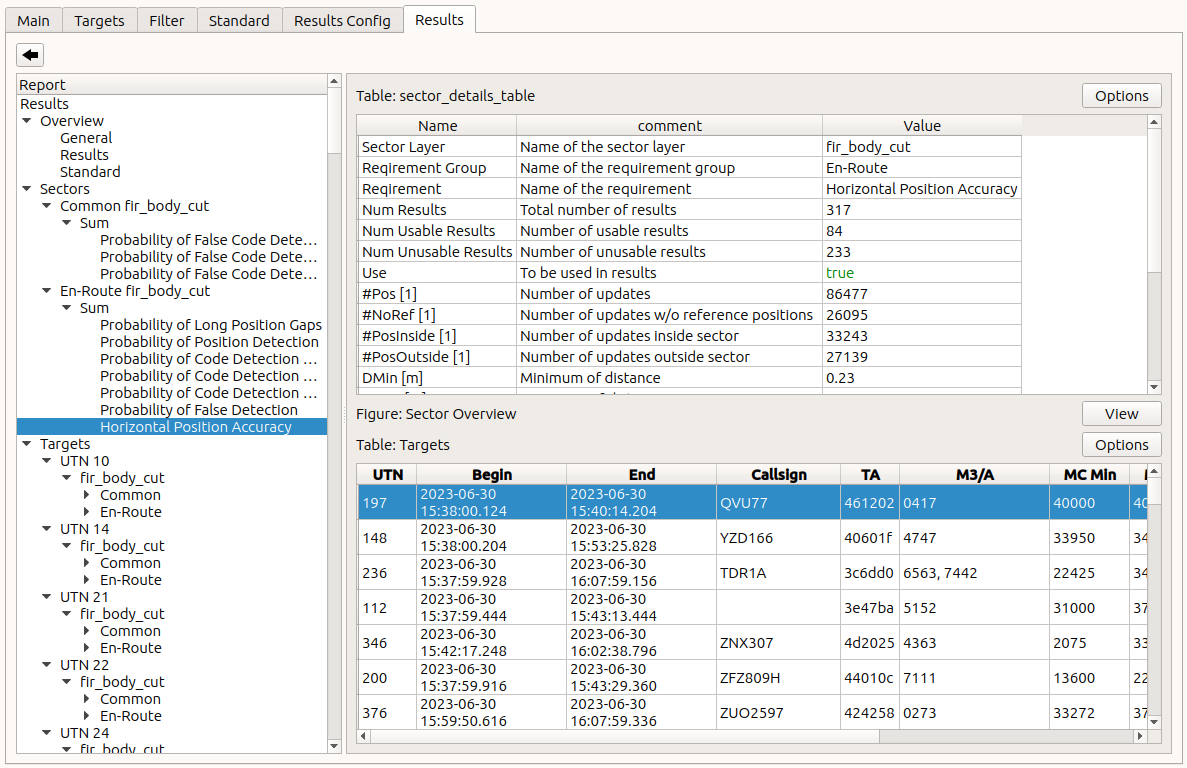
\includegraphics[width=18cm,frame]{figures/eval_results_sec_det_example.png}
  \caption{Evaluation results: Sector Detail Example}
\end{figure}

On the left side, the current position in the results sections is shown. On the right, the current results are shown. At the top, there is an overview table giving the details of the calculation results in the respective sector layer and requirement. \\

At the bottom, further result details are listed per-target, sorted in this example by the Probability of Detection (PD). \\

When left clicking a row, the respective target data and result errors are shown in the existing Geographic Views.

\begin{figure}[H]
  \hspace*{-2.5cm}
    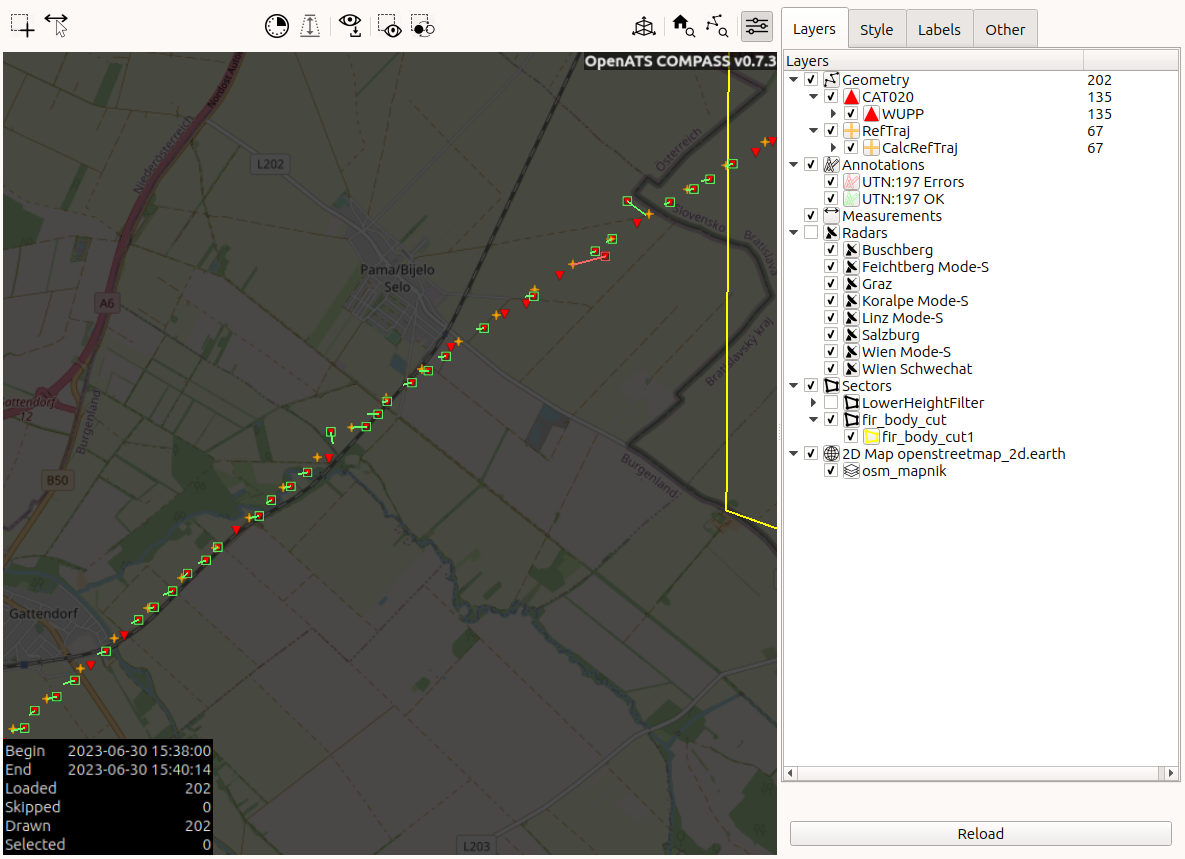
\includegraphics[width=19cm]{figures/eval_results_single_geoview.png}
  \caption{Evaluation results: PD Misses in Geographic View}
\end{figure}

When right-clicking a target, several options are shown:
\begin{itemize}  
\item Remove: Remove this specific target from the evaluation (giving a reason as comment)
\item Show full UTN: Load all data from the respective target (not just used reference / test data)
\item Show Surrounding Data: Load all data surrounding the target in position and time (e.g. to find association issues)
\end{itemize}  
\ \\

When double-clicking a row, a step into the respective target details is performed.

\subsection{Result Per-Target Details}

\begin{figure}[H]
  \hspace*{-2cm}
    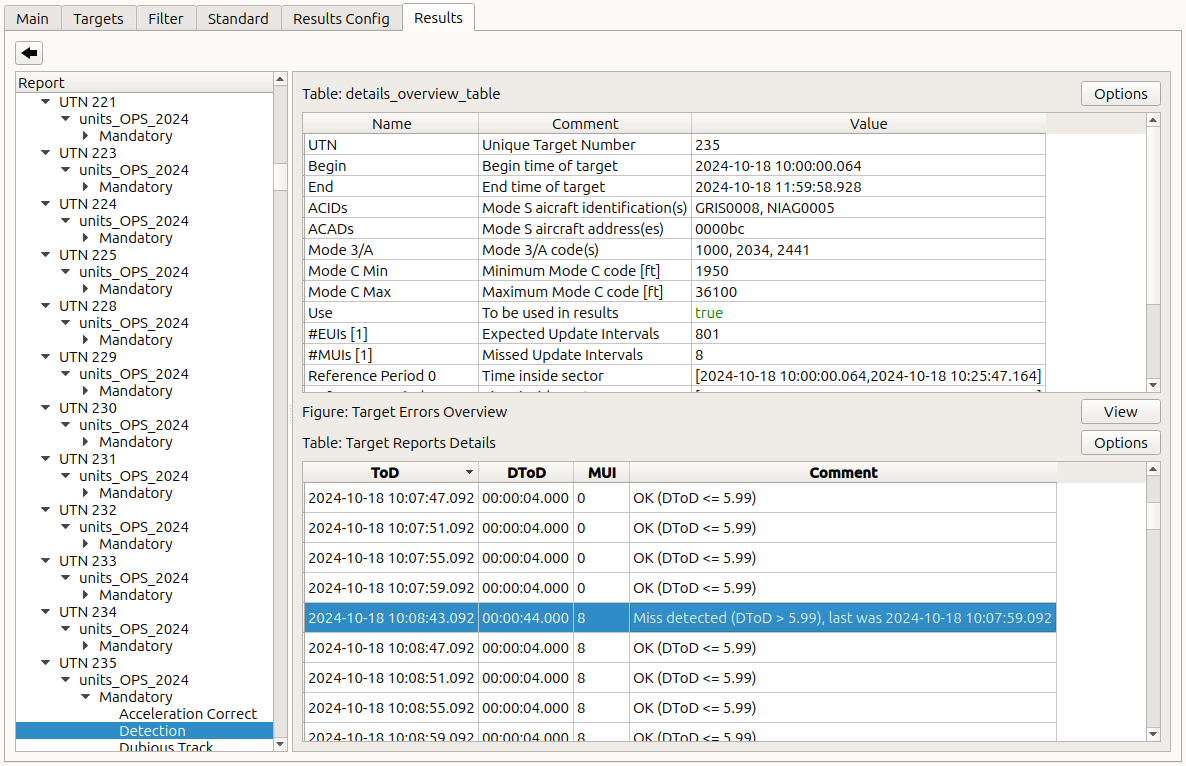
\includegraphics[width=18cm,frame]{figures/eval_results_target_example.png}
  \caption{Evaluation results: Per-Target Detail Example}
\end{figure}

On the left side, the current position in the results sections is shown. On the right, the current results are shown. At the top, there is an overview table giving the details of the calculation results for the target in the respective sector layer and requirement. \\

At the bottom, further result details are listed per-target-report, sorted in this example by time. \\

When single-clicking a row, the respective target data and the respective single result error are shown in the existing Geographic Views.

\begin{figure}[H]
  \hspace*{-2.5cm}
    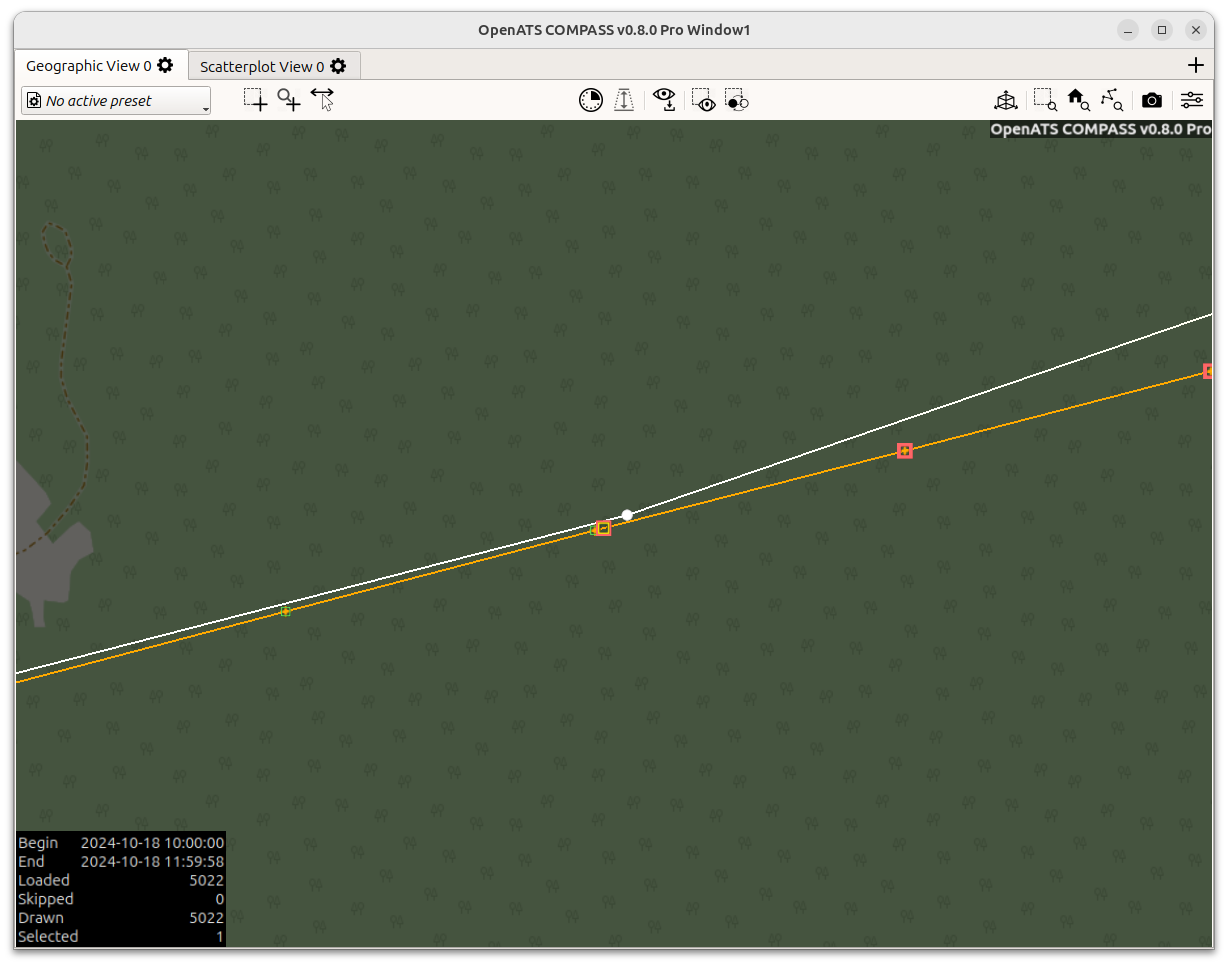
\includegraphics[width=19cm]{figures/eval_results_pd_single_tr_geoview.png}
  \caption{Evaluation results: Target Single PD Error in Geographic View}
\end{figure}

\subsection{Targets of Interest}
\label{sec:eval_targets_of_interest}

\begin{figure}[H]
  \hspace*{-2cm}
    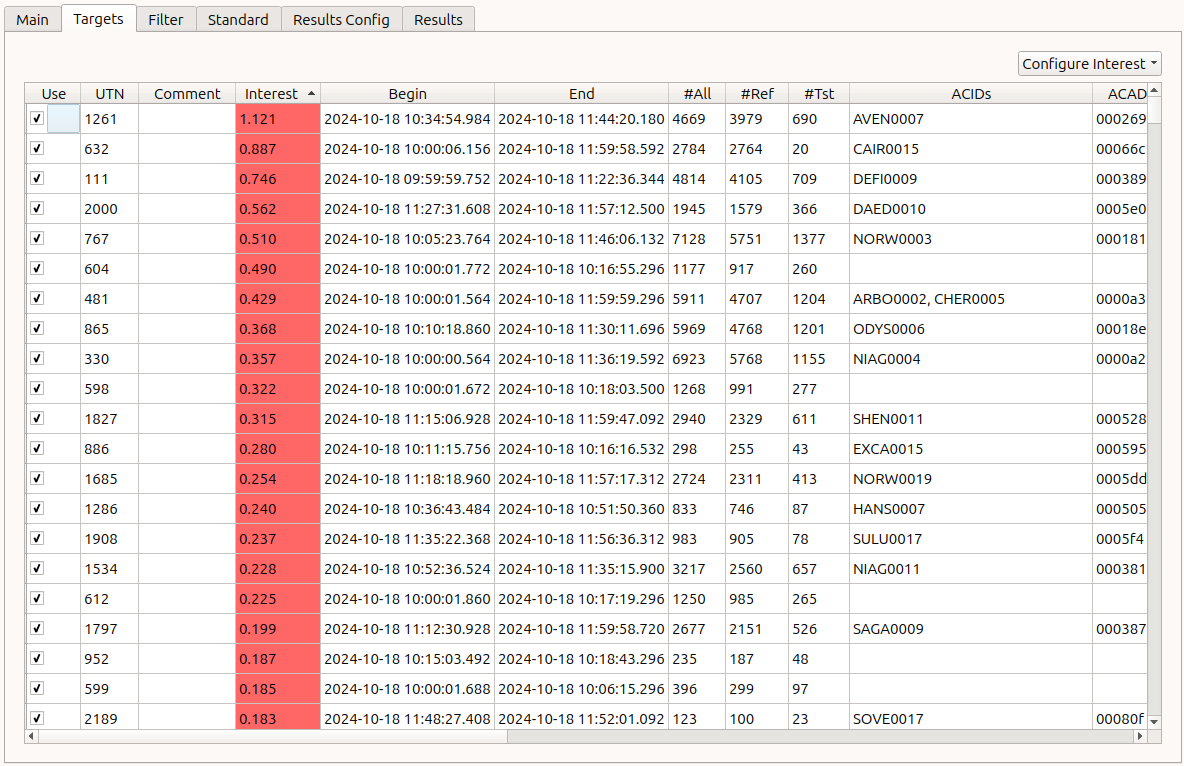
\includegraphics[width=18cm,frame]{figures/eval_targets_eval.png}
  \caption{Evaluation Targets tab with evaluated data}
\end{figure}

After running an evaluation, in the Evaluation Targets tab, the displayed interest is a numerical score showing how strong a negative impact a target had on all requirement results. \\

The interest factor is calculated by:
\begin{itemize}  
\item Stepping through all targets in all given sectors and requirements
\item For each target and requirement, the negative contribution of said target to the respective requirement is calculated
\begin{itemize}  
\item Resulting in a value between 0 (no negative impact) and 1 (all negative contributions come from this single target
\end{itemize}
\item For each target an accumulated sum of per-requirement interest factors is calculated
\end{itemize}
\ \\

The coloring is performed as follows:
\begin{itemize}  
\item higher than 0.1: red
\item higher than 0.05 and lower than 0.1: orange
\item 0.05 and below: green
\end{itemize}
\ \\

When right-clicking a target, several options are shown:
\begin{itemize}  
\item Show full UTN: Load all data from the respective target (not just used reference / test data)
\item Show Surrounding Data: Load all data surrounding the target in position and time (e.g. to find association issues)
\item Jump to requirement: Jump to the respective requirement results section
\end{itemize}
\ \\

Using the 'Configure Interest' button, a list of all requirements is given to select which interest values should be aggregated.
\begin{figure}[H]
  \hspace*{-2.5cm}
    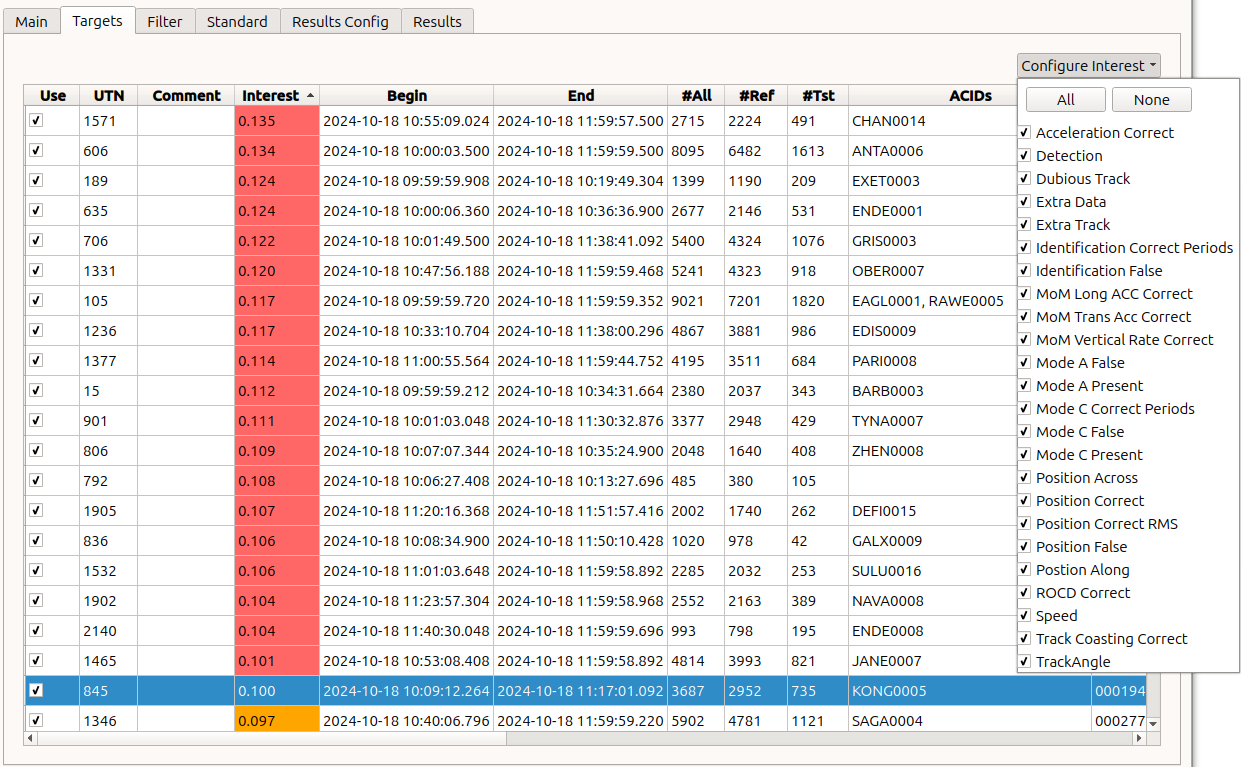
\includegraphics[width=19cm,frame]{figures/eval_targets_config_interest.png}
  \caption{Evaluation Targets: Configure Interest}
\end{figure}

